\section{Две геометрические теоремы о плоском движении}

\begin{theorem}[Шаля]
  \label{theorem:chasles}
  Всякое перемещение плоской фигуры в своей плоскости, а следовательно, и всякое
  плоское перемещение твёрдого тела можно себе представить как совокупность двух
  перемещений:
  \begin{enumerate}
    \item поступательного перемещения, зависящего от выбора полюса, и
    \item вращательного перемещения вокруг полюса;
  \end{enumerate}
  угол и направление поворота от выбора полюса не зависят.
\end{theorem}

\begin{proof}
  Положение плоской фигуры может быть задано положением двух её точек $O'$ и
  $M$ или положением отрезка $O'M$

  \begin{figure}[H]
    \centering
    \resizebox{\linewidth}{!}{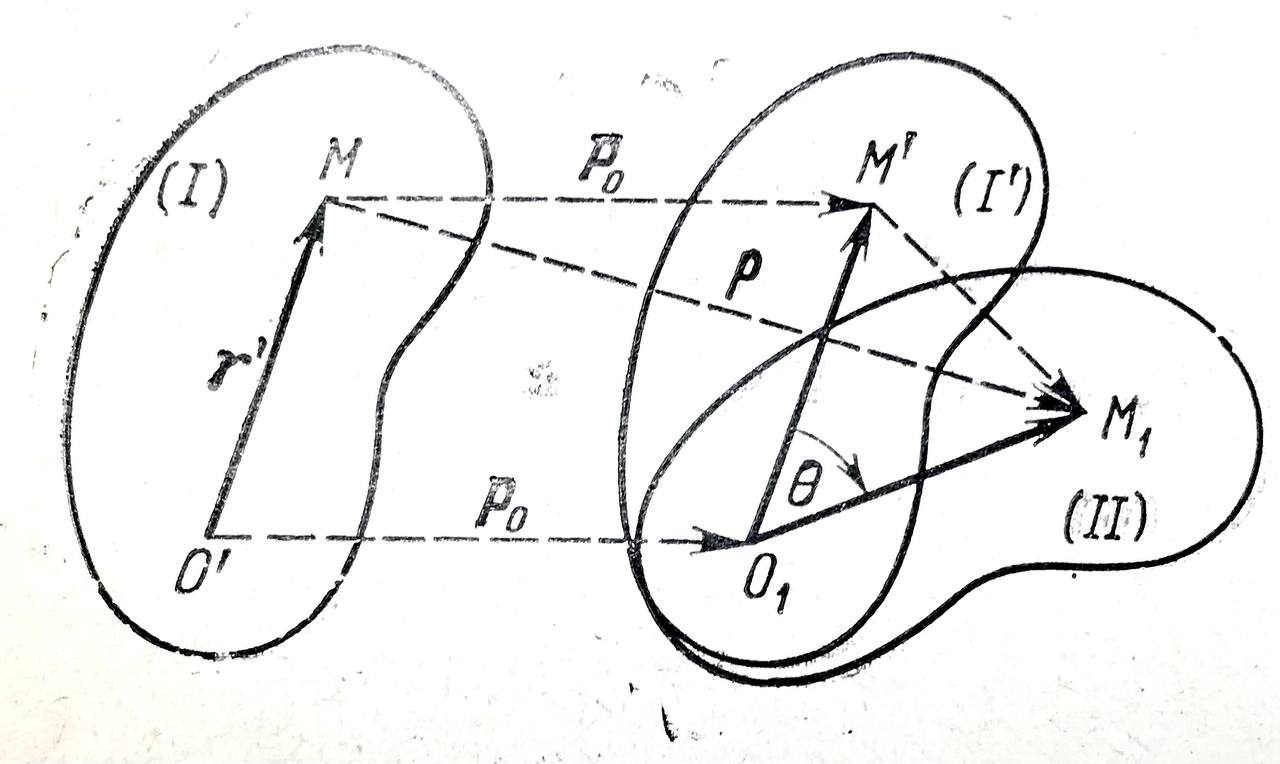
\includegraphics{src/mechanics/pictures/15_1.jpg}}

    \caption{}
    \label{fig:15_1}
  \end{figure}

  Пусть фигура $O'M$ переместилась из положения $I$ в положение $II$. Разобьём
  переход на две части. Сначала переместим фигуру поступательно в положение
  $I'$, причём все точки её получат перемещения, геометрические равные
  перемещению $\vv{O'O_1}$ полюса $O'$, а затем повернём фигуру на $\angle M'O_1
  M_1$ вокруг оси, проходящей через точку $O_1$ перпендикулярно к плоскости
  фигуры.

  Заметим, что вектор поступательного перемещения зависит от выбора полюса, а
  угол поворота не зависит от этого выбора. В самом деле, тот же переход из
  положения $I$ в положение $II$ можно осуществить, приняв за полюс точку $M$ и
  переместив сначала фигуру в положение $I''$, причём все точки фигуры получат
  перемещения, геометрически равные $\vv{M M_1}$ и отличные от $\vv{O' O_1}$,
  а затем повернув фигуру на $\angle O'' M_1 O_1$ вокруг оси, проходящей через
  $M_1$. Но по свойству поступательного перемещения $\vv{O'' M_1}$ параллелен
  $\vv{O' M}$ и точно так же $\vv{O_1 M'}$ параллелен $\vv{O'M}$. Следовательно,
  $\vv{O'' M_1}$ и $\vv{O_1 M'}$ параллельны между собой и
  $\angle O'' M_1 O = \angle M' O_1 M_1$. Вместе с тем поворот вокруг точек
  $O_1$ и $M_1$ в том и другом случае происходит в одну и ту же сторону.
  Окончательное положение фигуры не зависит от того, будет ли сначала
  совершаться поступательное перемещение или поворот.

  \begin{figure}[H]
    \centering
    \resizebox{\linewidth}{!}{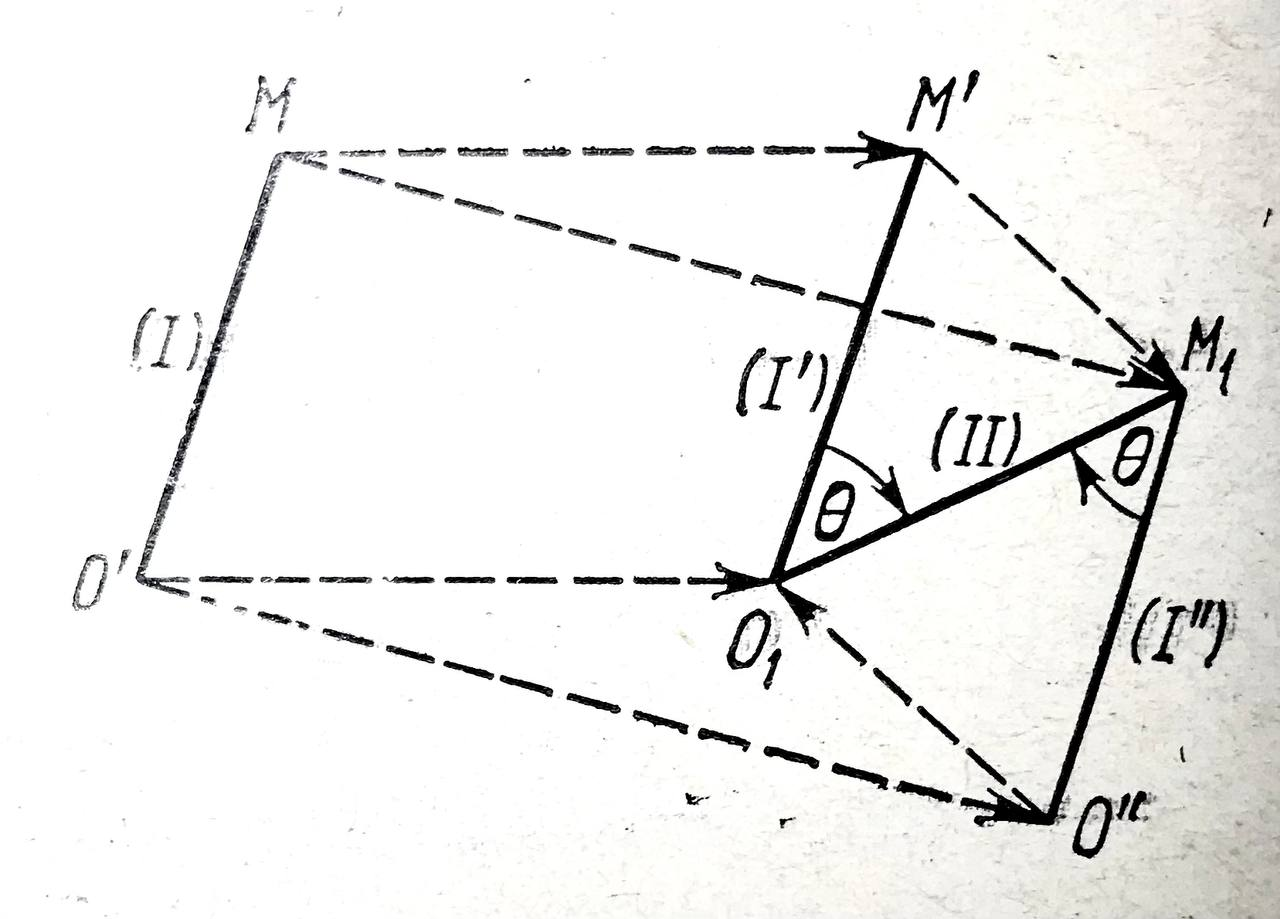
\includegraphics{src/mechanics/pictures/15_2.jpg}}

    \caption{}
    \label{fig:15_2}
  \end{figure}
\end{proof}

Естественно возникает вопрос, нельзя ли, используя произвольность в выборе
полюса, осуществить заданное перемещение тела \textit{одним} поворотом, без
поступательного перемещения.

На этот вопрос даёт ответ
\begin{theorem}[Эйлера]
  \label{theorem:euler}
  Всякое непоступательное перемещение плоской фигуры в её плоскости может быть
  осуществлено одним поворотом вокруг некоторого центра.
\end{theorem}

\begin{proof}
  \begin{figure}[H]
    \centering
    \resizebox{\linewidth}{!}{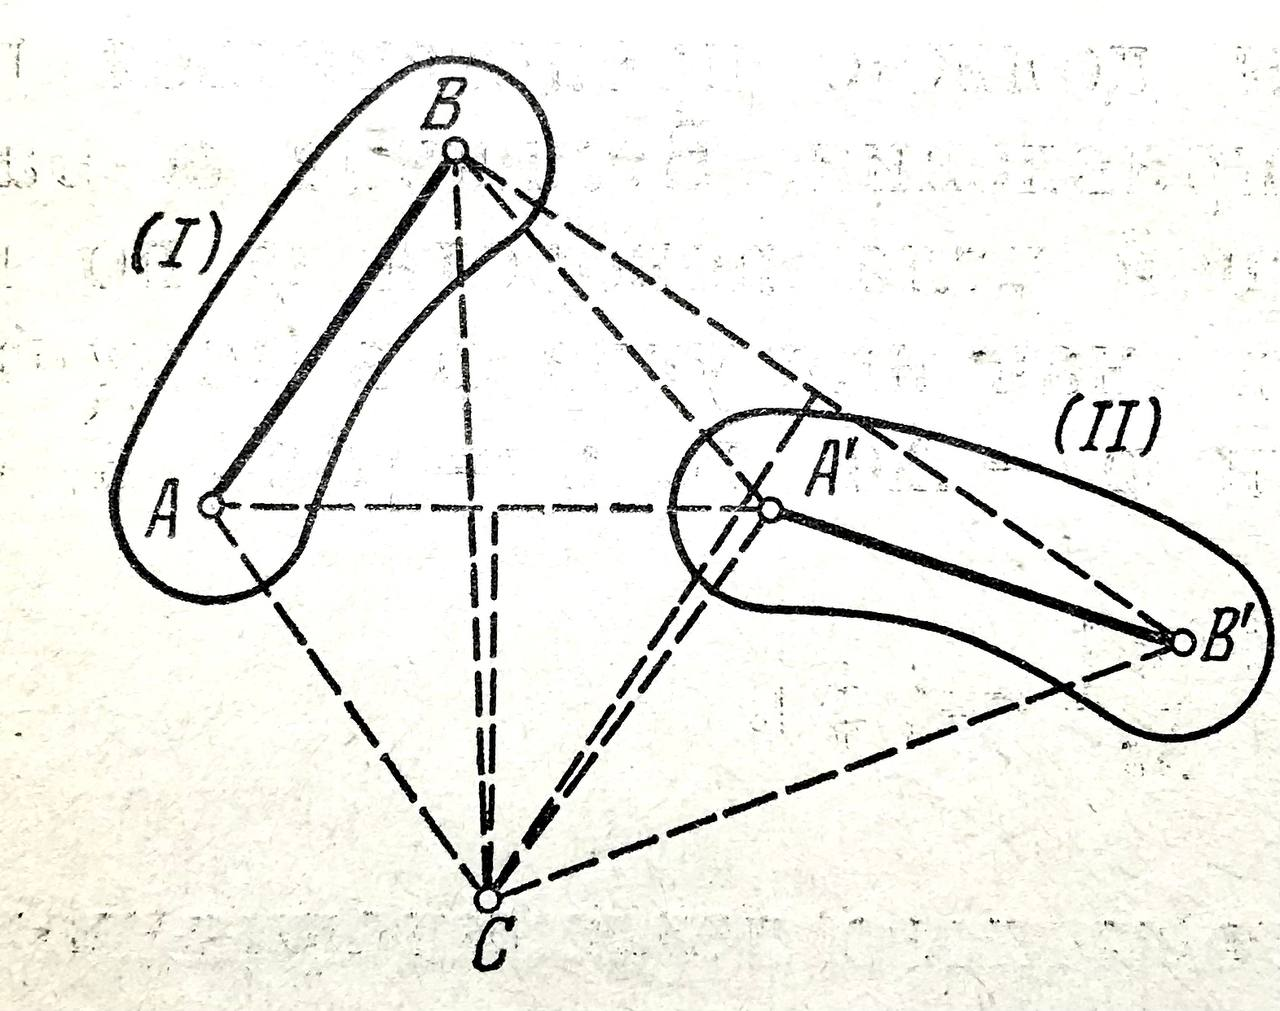
\includegraphics{src/mechanics/pictures/15_3.jpg}}

    \caption{}
    \label{fig:15_3}
  \end{figure}

  Пусть фигура переместилась из положения $I$ в положение $II$.

  Восставим из середин перемещений точек $A$ и $B$, то есть из середин отрезков
  $AA'$ и $BB'$, перпендикуляры и найдём пересечение их в точке $C$.

  Докажем, что фигура $I$ может быть переведена в положение $II$ поворотом
  вокруг центра $C$ на $\angle ACA' = \angle BCB'$. В самом деле, треугольники
  $ABC$ и $A'CB'$ равны между собой, так как $AB = A'B'$ в силу неизменяемости
  фигуры и $AC = A"C,~BC = B'C$ по построению. Следовательно,
  \begin{equation*}
    \angle ACB = \angle A'CB';
  \end{equation*}
  прибавляя к обеим частям этого равенства по одинаковому углу $BCA'$, найдём,
  что
  \begin{equation*}
    \angle ACA' = \angle BCB'.
  \end{equation*}

  Повернём теперь фигуру $I$ на угол $ACA'$, тогда $AC$ совместится с $A'C$,
  $BC$ --- с $B'C$, так как углы равны, и $AB$ совместится с $A'B'$, что и
  доказывает теорему.
\end{proof}

\begin{definition}
  Точка $C$ называется \textit{центром поворота}.
\end{definition}

\begin{remark}
  Только что указанное построение не даёт результата в двух случаях:
  \begin{enumerate}
    \item если перпендикуляры, восстановленные из середин перемещений, сливаются
      в одну линию, но в этом случае центр поворота лежит на пересечении
      продолжений отрезков $AB$ и $A'B'$;

      \begin{figure}[H]
        \centering
        \resizebox{\linewidth}{!}
          {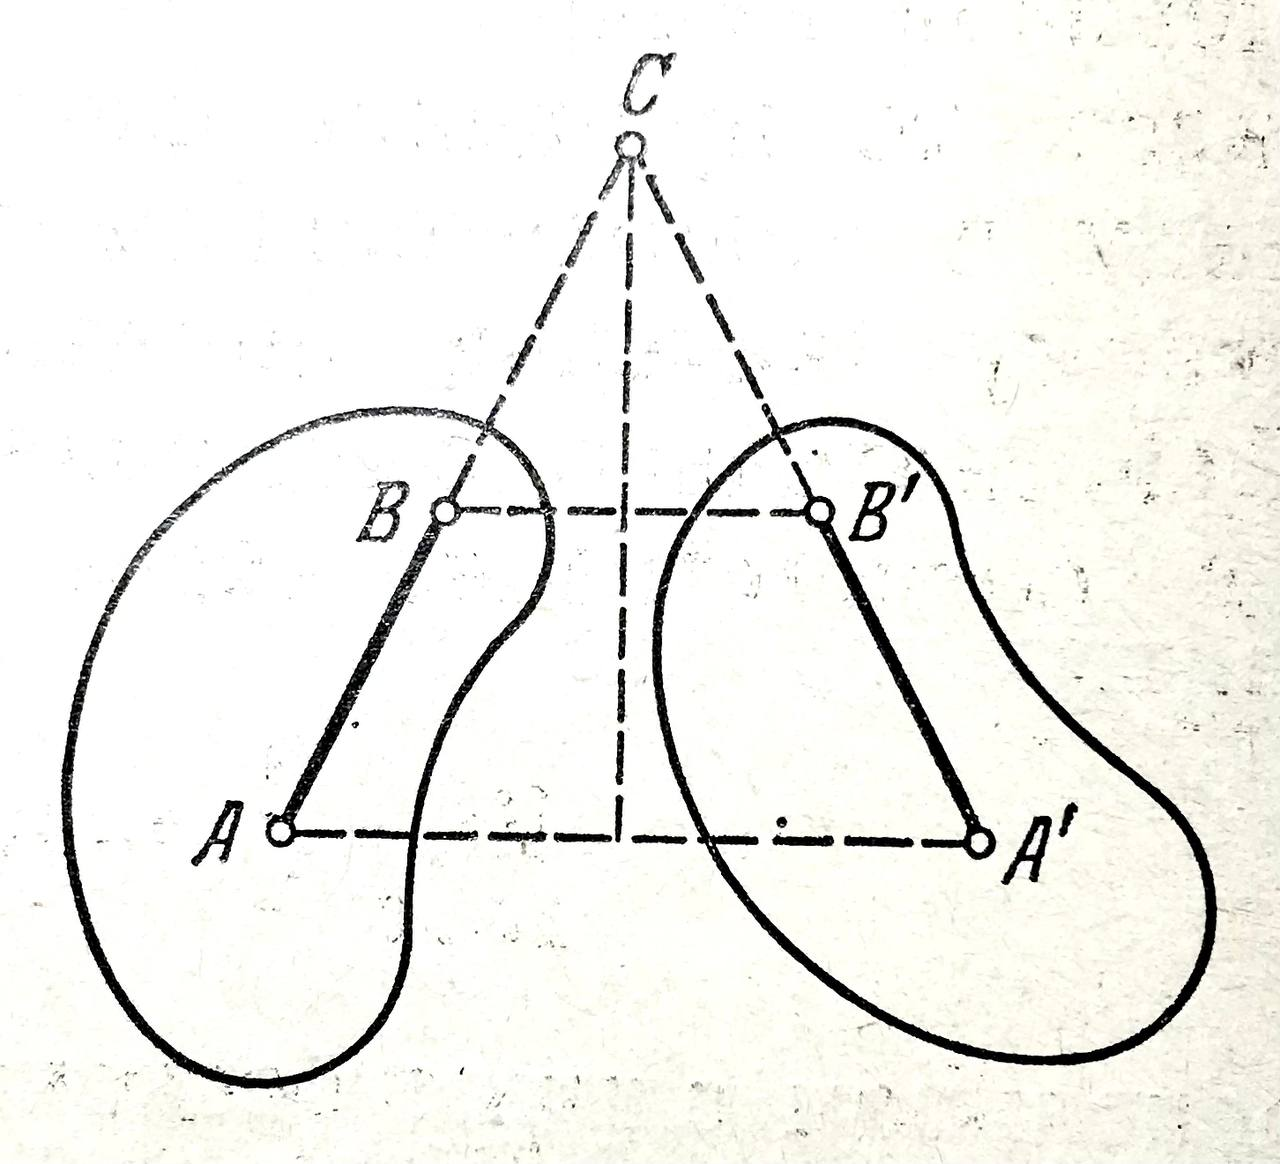
\includegraphics{src/mechanics/pictures/15_4.jpg}}

        \caption{}
        \label{fig:15_4}
      \end{figure}

    \item если перпендикуляры параллельны между собой, что имеет место при
      \textit{поступательном} перемещении; этот случай соответствует положению
      центра поворота в бесконечном удалении.
  \end{enumerate}

\end{remark}

\subsection{Список литературы}
\begin{enumerate}
  \item \cite{lourie}
\end{enumerate}

